\section{Auswertung} 

\begin{align} 
    \intertext{Im ersten Teil des Versuches wird die Verdampfungswärme $L$ bestimmt. 
    Der Umgebungsdruck beträgt}
    p_{0} = 1023\,\unit{\milli\bar} = 1023 \cdot 10^{2}\,\unit{\pascal} \,. \notag \\
    \intertext{Die hergeleitete Formel zur Berechnung der Verdampfungswärme, mit Hilfe aus der Formel (\ref{5}), lautet}
    \ln\left(\frac{p}{p_{0}}\right) = -\frac{L}{R} \cdot \frac{1}{T}\,. \label{6}
    \intertext{Die Wertepaare aus der Tabelle \ref{Tabelle1} und \ref{Tabelle2} werden in einem Verhältnis zueinander gebracht, dazu wird der Logarithmus vom Druck zum Umgebungsdruck gegen den Kehrwert der Temperatur aufgestellt
    und in Abbildung \ref{Abbildung5} dargestellt.}
    \notag
\end{align}

\begin{table}[H]    
    \centering
    \caption{Messwerte des ersten Versuches.} 
    \label{Tabelle1}
    \begin{tabular} {c|  c|  c|  c}
        \toprule
        {$ p \mathbin{/} 10^{2}\, \unit{\pascal} $} &
        {$ \text{T} \mathbin{/} \unit{\kelvin} $} &
        {$ \ln \left(\frac{p}{p_{0}}\right) $} &
        {$ \frac{1}{\text{T}} \mathbin{/} 10^{-3}\,\frac{1}{\unit{\kelvin}} $} \\
        \midrule
        23  & 291,15 & -3,79 & 3,43 \\
        31  & 291,15 & -3,49 & 3,43 \\
        34  & 292,15 & -3,40 & 3,42 \\
        45  & 296,15 & -3,12 & 3,37 \\
        65  & 304,15 & -2,75 & 3,28 \\
        85  & 311,15 & -2,48 & 3,21 \\
        105 & 316,15 & -2,27 & 3,16 \\
        125 & 321,15 & -2,10 & 3,11 \\
        145 & 325,15 & -1,95 & 3,07 \\
        165 & 327,65 & -1,82 & 3,05 \\
        185 & 330,15 & -1,71 & 3,02 \\
        205 & 332,15 & -1,60 & 3,01 \\
        225 & 334,65 & -1,51 & 2,98 \\
        245 & 338,15 & -1,42 & 2,97 \\
        265 & 339,65 & -1,35 & 2,95 \\
        285 & 341,65 & -1,27 & 2,94 \\
        305 & 342,65 & -1,21 & 2,93 \\
        325 & 342,65 & -1,14 & 2,91 \\
        345 & 344,15 & -1,08 & 2,90 \\
        365 & 346,15 & -1,03 & 2,88 \\
        385 & 347,15 & -0,97 & 2,88 \\
        405 & 348,15 & -0,92 & 2,87 \\
        425 & 349,15 & -0,87 & 2,86 \\
        445 & 351,15 & -0,83 & 2,84 \\
        465 & 352,15 & -0,78 & 2,83 \\
        485 & 353,15 & -0,74 & 2,83 \\
        505 & 354,15 & -0,70 & 2,82 \\
        525 & 354,65 & -0,66 & 2,81 \\
        545 & 356,15 & -0,62 & 2,80 \\
        565 & 357,15 & -0,59 & 2,79 \\
        585 & 357,65 & -0,55 & 2,79 \\
        605 & 359,15 & -0,52 & 2,78 \\
        625 & 360,15 & -0,49 & 2,77 \\
        645 & 361,15 & -0,46 & 2,76 \\
        \bottomrule
    \end{tabular} 
\end{table}


\begin{table}[H]    
    \centering
    \caption{Messwerte des ersten Versuches.} 
    \label{Tabelle2}
    \begin{tabular} {c|  c|  c|  c}
        \toprule
        {$ p \mathbin{/} 10^{-3}\, \unit{\bar} $} &
        {$ \text{T} \mathbin{/} \unit{\kelvin} $} &
        {$ \ln \left(\frac{p}{p_{0}}\right) $} &
        {$ \frac{1}{\text{T}} \mathbin{/} 10^{-3}\,\frac{1}{\unit{\kelvin}} $} \\
        \midrule
        665 & 361,65 & -0,43 & 2,76 \\
        685 & 362,15 & -0,40 & 2,76 \\
        705 & 363,15 & -0,37 & 2,75 \\
        725 & 364,15 & -0,34 & 2,74 \\
        745 & 365,15 & -0,31 & 2,73 \\
        765 & 365,65 & -0,29 & 2,73 \\
        785 & 366,15 & -0,26 & 2,73 \\
        805 & 367,15 & -0,23 & 2,72 \\
        825 & 367,65 & -0,21 & 2,71 \\
        845 & 368,15 & -0,19 & 2,71 \\
        865 & 369,15 & -0,16 & 2,70 \\
        885 & 369,65 & -0,14 & 2,70 \\
        905 & 310,15 & -0,12 & 2,70 \\
        925 & 370,65 & -0,10 & 2,69 \\
        945 & 371,15 & -0,07 & 2,69 \\
        965 & 371,65 & -0,05 & 2,69 \\
        985 & 372,15 & -0,03 & 2,68 \\
        1002 & 373,15 & -0,01 & 2,67 \\
        \bottomrule
    \end{tabular} 
\end{table}

\begin{figure}[H]
    \centering
    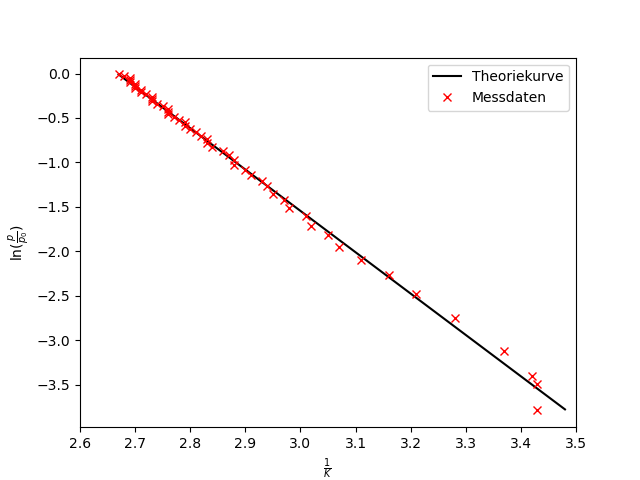
\includegraphics[height=80mm]{bilder/plot1.png}
    \caption{Die Lineare Regression der Datenpaare bis 1 bar.\label{Abbildung5} }
\end{figure}

\begin{align}
    \intertext{Die Ausgleichsgerade liefert}
    a = (-2.14 \pm 0.01) \cdot 10^{3}\,\unit{\kelvin} \notag \\
    b = (2.668 \pm 0.002)\,. \notag \\
    \intertext{Durch die Gleichung (\ref{5}) und die Ausgleichsgerade lässt sich die Verdampfungswärme durch die Funktion}
    a = -\frac{L}{R} \to L = -a \cdot R \label{7} \\
    \intertext{bestimmen. Daraus folgt}
    L = ( 17.79 \pm 0.083 ) \cdot 10^{3}\,\frac{\text{J}}{\text{mol}}. \notag\\
    \intertext{Für die Volumenarbeit $W = p \cdot V$, wofür die äußere Verdampfungsenergie $L_{a}$ benötigt wird, um das Volumen eines Mols der Flüssigkeit auf das Volumen eines Gases zu vergrößern,
    lässt sich mit der idealen Gasgleichung aus der Formel (\ref{1}) gleichsetzen. Somit folgt mit der Temperatur $T = 373\,\unit{\kelvin}$: }
    L_{a} = W = pV = RT \label{8} \\
    = 3.101 \cdot 10^{3}\,\frac{\text{J}}{\text{mol}}\,. \notag \\
    \intertext{Anschließend für die innere Energie $L_{i}$}
    L_{i} = L - L_{a} \label{9}\\
    = (14.689 \pm 0.520) \cdot 10^{3}\,\frac{\text{J}}{\text{mol}}\,. \notag\\
    \intertext{Die Energie wird benötigt, um die molekulare Bindungskräft zu überwinden. 
    Zur Verdeutlichung der inneren Energie pro Molekül wird die innere Energie durch die Avogadro-Konstante $N_{A} = 6.022 \cdot 10^{23}\,\frac{1}{\text{mol}}$ geteilt. 
    Zudem wird das Ergebnis in Elektronenvolt angegeben. Das führt zu}
    L_{i} = (0,152 \pm 0,004 )\,\text{eV}\,. \notag
\end{align}

\subsection{Messung von 1 bis 15 bar}

\begin{flushleft}
    Die Messung wird mit der Apparatur aus Abbildung \ref{Abbildung4} durchgeführt.
    Dabei wird die Verdampfungswärme in Abhängigkeit der Temperatur bestimmt.
    Dafür wird die Gleichung (\ref{4}) benötigt und umgestellt zu 
\end{flushleft}

\begin{align} 
    L = T(V_{\text{D}} - V_{\text{F}})\, \frac{\text{d}p}{\text{d}T}\,. \label{10}
    \intertext{Es ist zu beachten, dass sich $V_{\text{D}}$ nicht mehr durch die Gasgleichung aus der Formel (\ref{1}) ausdrücken lässt:}
    \left(p + \frac{A}{V_{\text{D}}^2}\right)\,\,V_{\text{D}} = RT \notag \\
    V_{\text{D}} = \frac{RT}{2p} \pm \sqrt{\frac{R^2T^2}{4p^2} - \frac{A}{p}} \\
    \text{mit}\,\, A = 0.9\,\frac{\unit{\joule\meter^3}}{\text{mol}^2} \notag
\end{align}

\begin{align}
    \intertext{Durch die Formel (\ref{10}) folgt}
    L = T \left[\frac{RT}{2p} \pm \sqrt{\frac{R^2T^2}{4p^2} - \frac{A}{P}}\right]\,\, \frac{\text{d}p}{\text{d}T} \notag \\
    = \frac{T}{p} \left[\frac{RT}{2} \pm \sqrt{\left(\frac{RT}{2}\right)^2 - Ap}\right]\,\, \frac{\text{d}p}{\text{d}T}\,. \label{12}
    \intertext{Zudessen, wird ein Ausgleichspolynom dritten Grades aufgestellt, um $\frac{\text{d}p}{\text{d}T}$ auszudrücken.} \notag
\end{align}

\begin{table}[H]
    \centering
    \caption{Messwerte des zweiten Versuches.} 
    \label{Tabelle3}
    \begin{tabular} {c  c || c  c}
        \toprule
        {$ p \mathbin{/} \cdot 10^{5}\unit{\pascal} $} &
        {$ T \mathbin{/} \unit{\kelvin} $} &
        {$ p \mathbin{/} \cdot 10^{5}\unit{\pascal} $} &
        {$ T \mathbin{/} \unit{\kelvin} $} \\
        \midrule
        0,5  & 367,65 & 8,0  & 443,15 \\
        1,0  & 381,15 & 8,5  & 445,15 \\
        1,5  & 391,65 & 9,0  & 447,15 \\
        2,0  & 393,15 & 9,5  & 449,15 \\
        2,5  & 404,15 & 10,0 & 452,15 \\
        3,0  & 411,15 & 10,5 & 453,15 \\
        3,5  & 415,15 & 11,0 & 456,15 \\
        4,0  & 420,15 & 11,5 & 458,15 \\
        4,5  & 423,15 & 12,0 & 459,15 \\
        5,0  & 426,15 & 12,5 & 461,15 \\
        5,5  & 429,15 & 13,0 & 463,15 \\
        6,0  & 432,15 & 13,5 & 465,15 \\
        6,5  & 435,15 & 14,0 & 466,15 \\
        7,0  & 438,15 & 14,5 & 467,15 \\
        7,5  & 440,15 & 15,0 & 468,15 \\
        \bottomrule
    \end{tabular} 
\end{table}

\begin{figure}[H]  
    \centering
    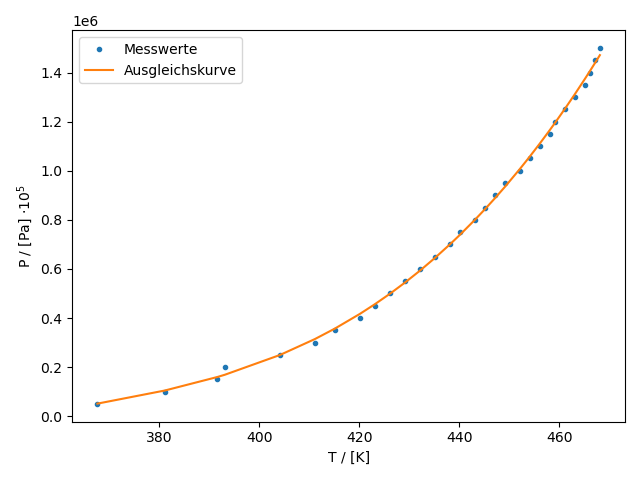
\includegraphics[height=80mm]{bilder/plot2.png}
    \caption{Das Ausgleichspolynom aus den Messpaaren.\label{Abbildung6} }
\end{figure}

\begin{align}
    \intertext{Dabei hat das Polynom die Form:}
    P(T) = aT^{3} + bT^{2} +cT + d \label{13} \\
    \frac{dp}{dT} = 3aT^{2} + 2bT + c \label{14} \\
    a = (0.8308 \pm -0.1187) \frac{\unit{\pascal}}{\unit{\kelvin}^3}  \notag\\
    b = ( -8.9432 \pm 1.5020 ) \cdot 10^{2}\,\frac{\unit{\pascal}}{\unit{\kelvin}^2}   \notag\\
    c = ( 3.2418 \pm -0.6313 ) \cdot 10^{5}\,\frac{\unit{\pascal}}{\unit{\kelvin}} \notag\\
    d = ( -3.9544 \pm -8.8206 ) \cdot 10^{7}\,\unit{\pascal}\,.  \notag
\end{align}
\begin{align}
    \intertext{Die zwei Gleichungen, (\ref{13}) und (\ref{14}), werden in die Formel (\ref{12}) eingesetzt und anschließend umgeformt zu}
    L(T) = \left[ \frac{RT}{2} \pm \sqrt{\left(\frac{RT}{2}\right)^2 - A \cdot\left(aT^{3}+bT^{2}+cT+d\right)} \right] \cdot \frac{3aT^{3}+2bT^{2}+cT}{aT^{3}+bT^{2}+cT+d}\, .
\end{align}

\begin{figure}[H]       
    \centering
    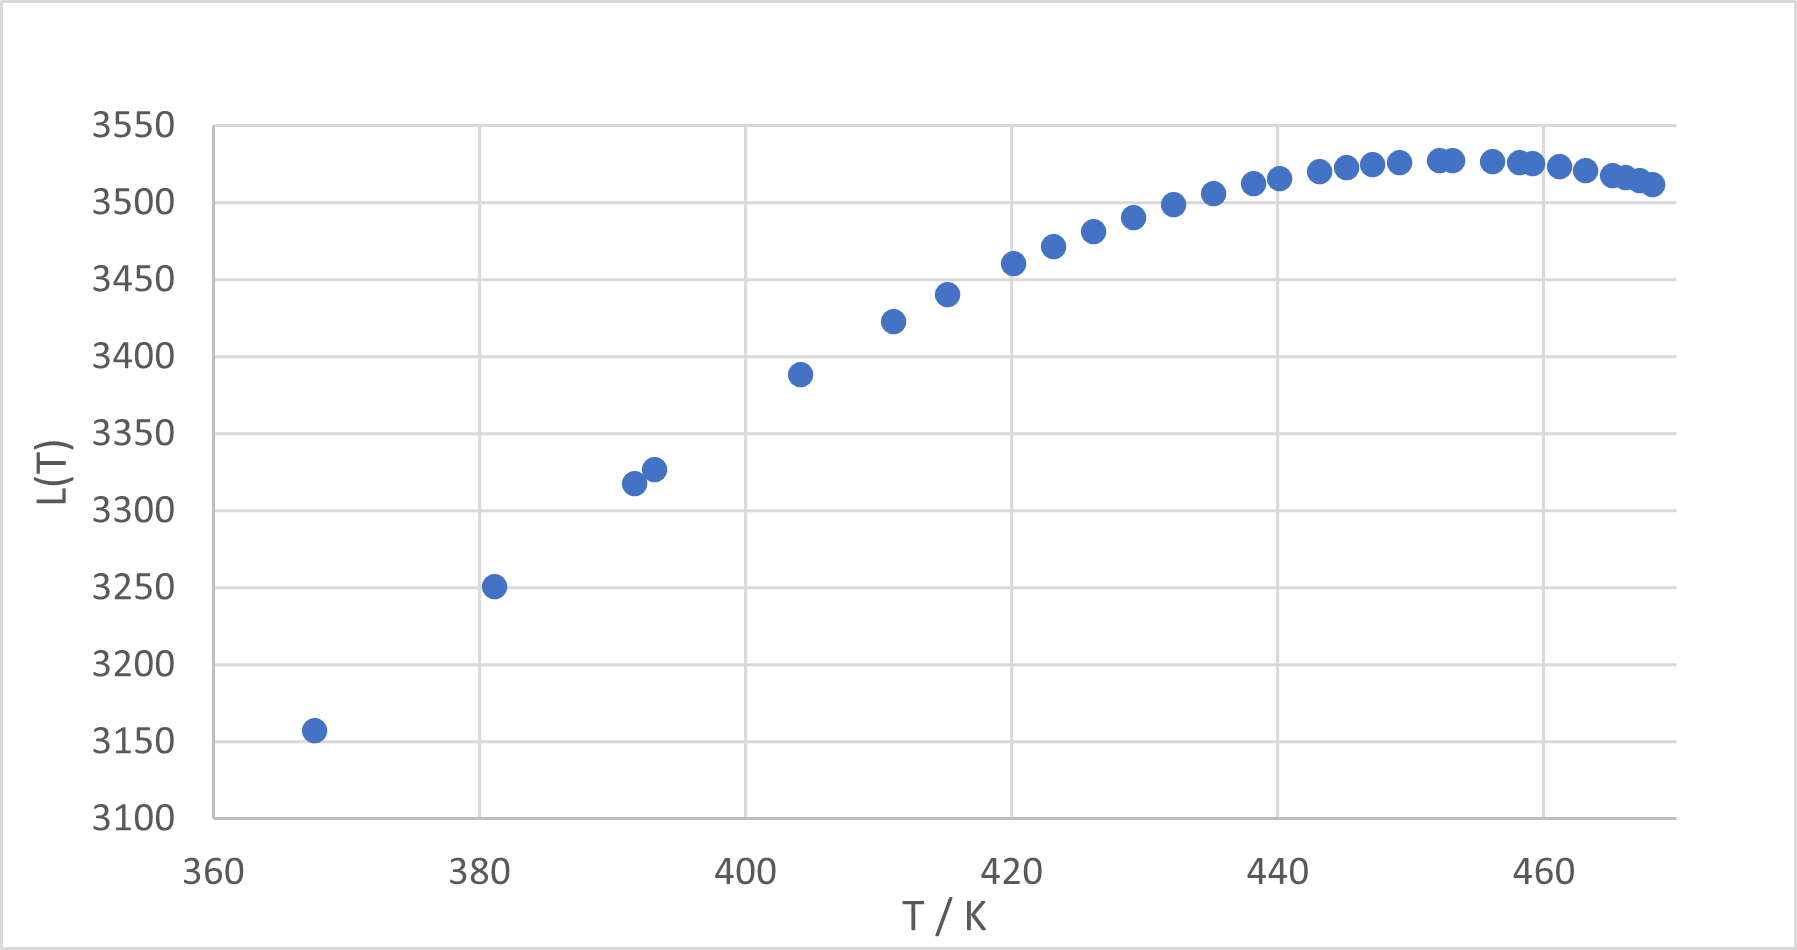
\includegraphics[height=55mm]{bilder/plot3.png}
    \caption{Verdampfungswärme erster Fall für Addition der Wurzel.\label{Abbildung7} }
\end{figure}

\begin{figure}[H]
    \centering
    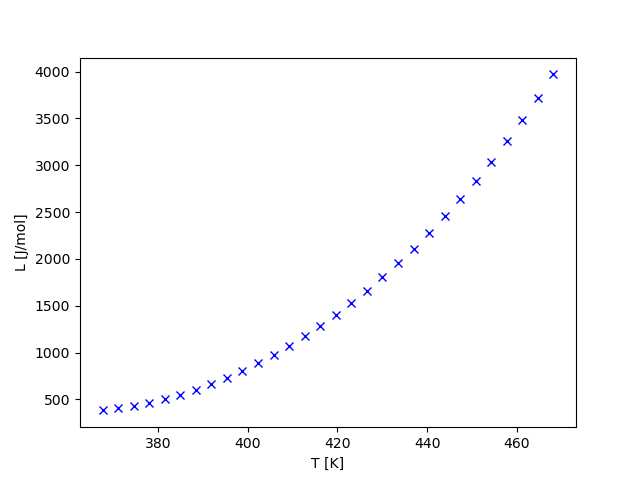
\includegraphics[height=80mm]{bilder/plot4.png}
    \caption{Verdampfungswärme zweiter Fall für Subtraktion der Wurzel.\label{Abbildung8} }
\end{figure}